\chapter{Indexation et recherche dans la collection CACM avec Lucene}

\section{Indexation}

Voir code sources attachés en annexe.

\section{Utilisation de différents \texttt{Analyzers}}

Lucene implémente plusieurs \texttt{Analyzers} pour traiter un document. Nous allons en essayer quelques-uns pour l'indexation et la recherche.

Voici les cinq questions auxquelles il faut répondre pour chaque \texttt{Analyzer} :

\begin{enumerate}
    \item The number of indexed documents and indexed terms.
    \item The number of indexed terms in the summary field.
    \item The top 10 frequent terms of the summary field in the index.
    \item The size of the index on disk.
    \item The required time for indexing.
\end{enumerate}

\subsection{WhitespaceAnalyzer}
\begin{enumerate}
    \item 3'203 / 38'029
    \item 26'821
    \item of / the / is / a / and / to / in / for / The / are
    \item 2'937 kB
    \item 2'347 ms
\end{enumerate}

\begin{figure}[H]
    \centering
    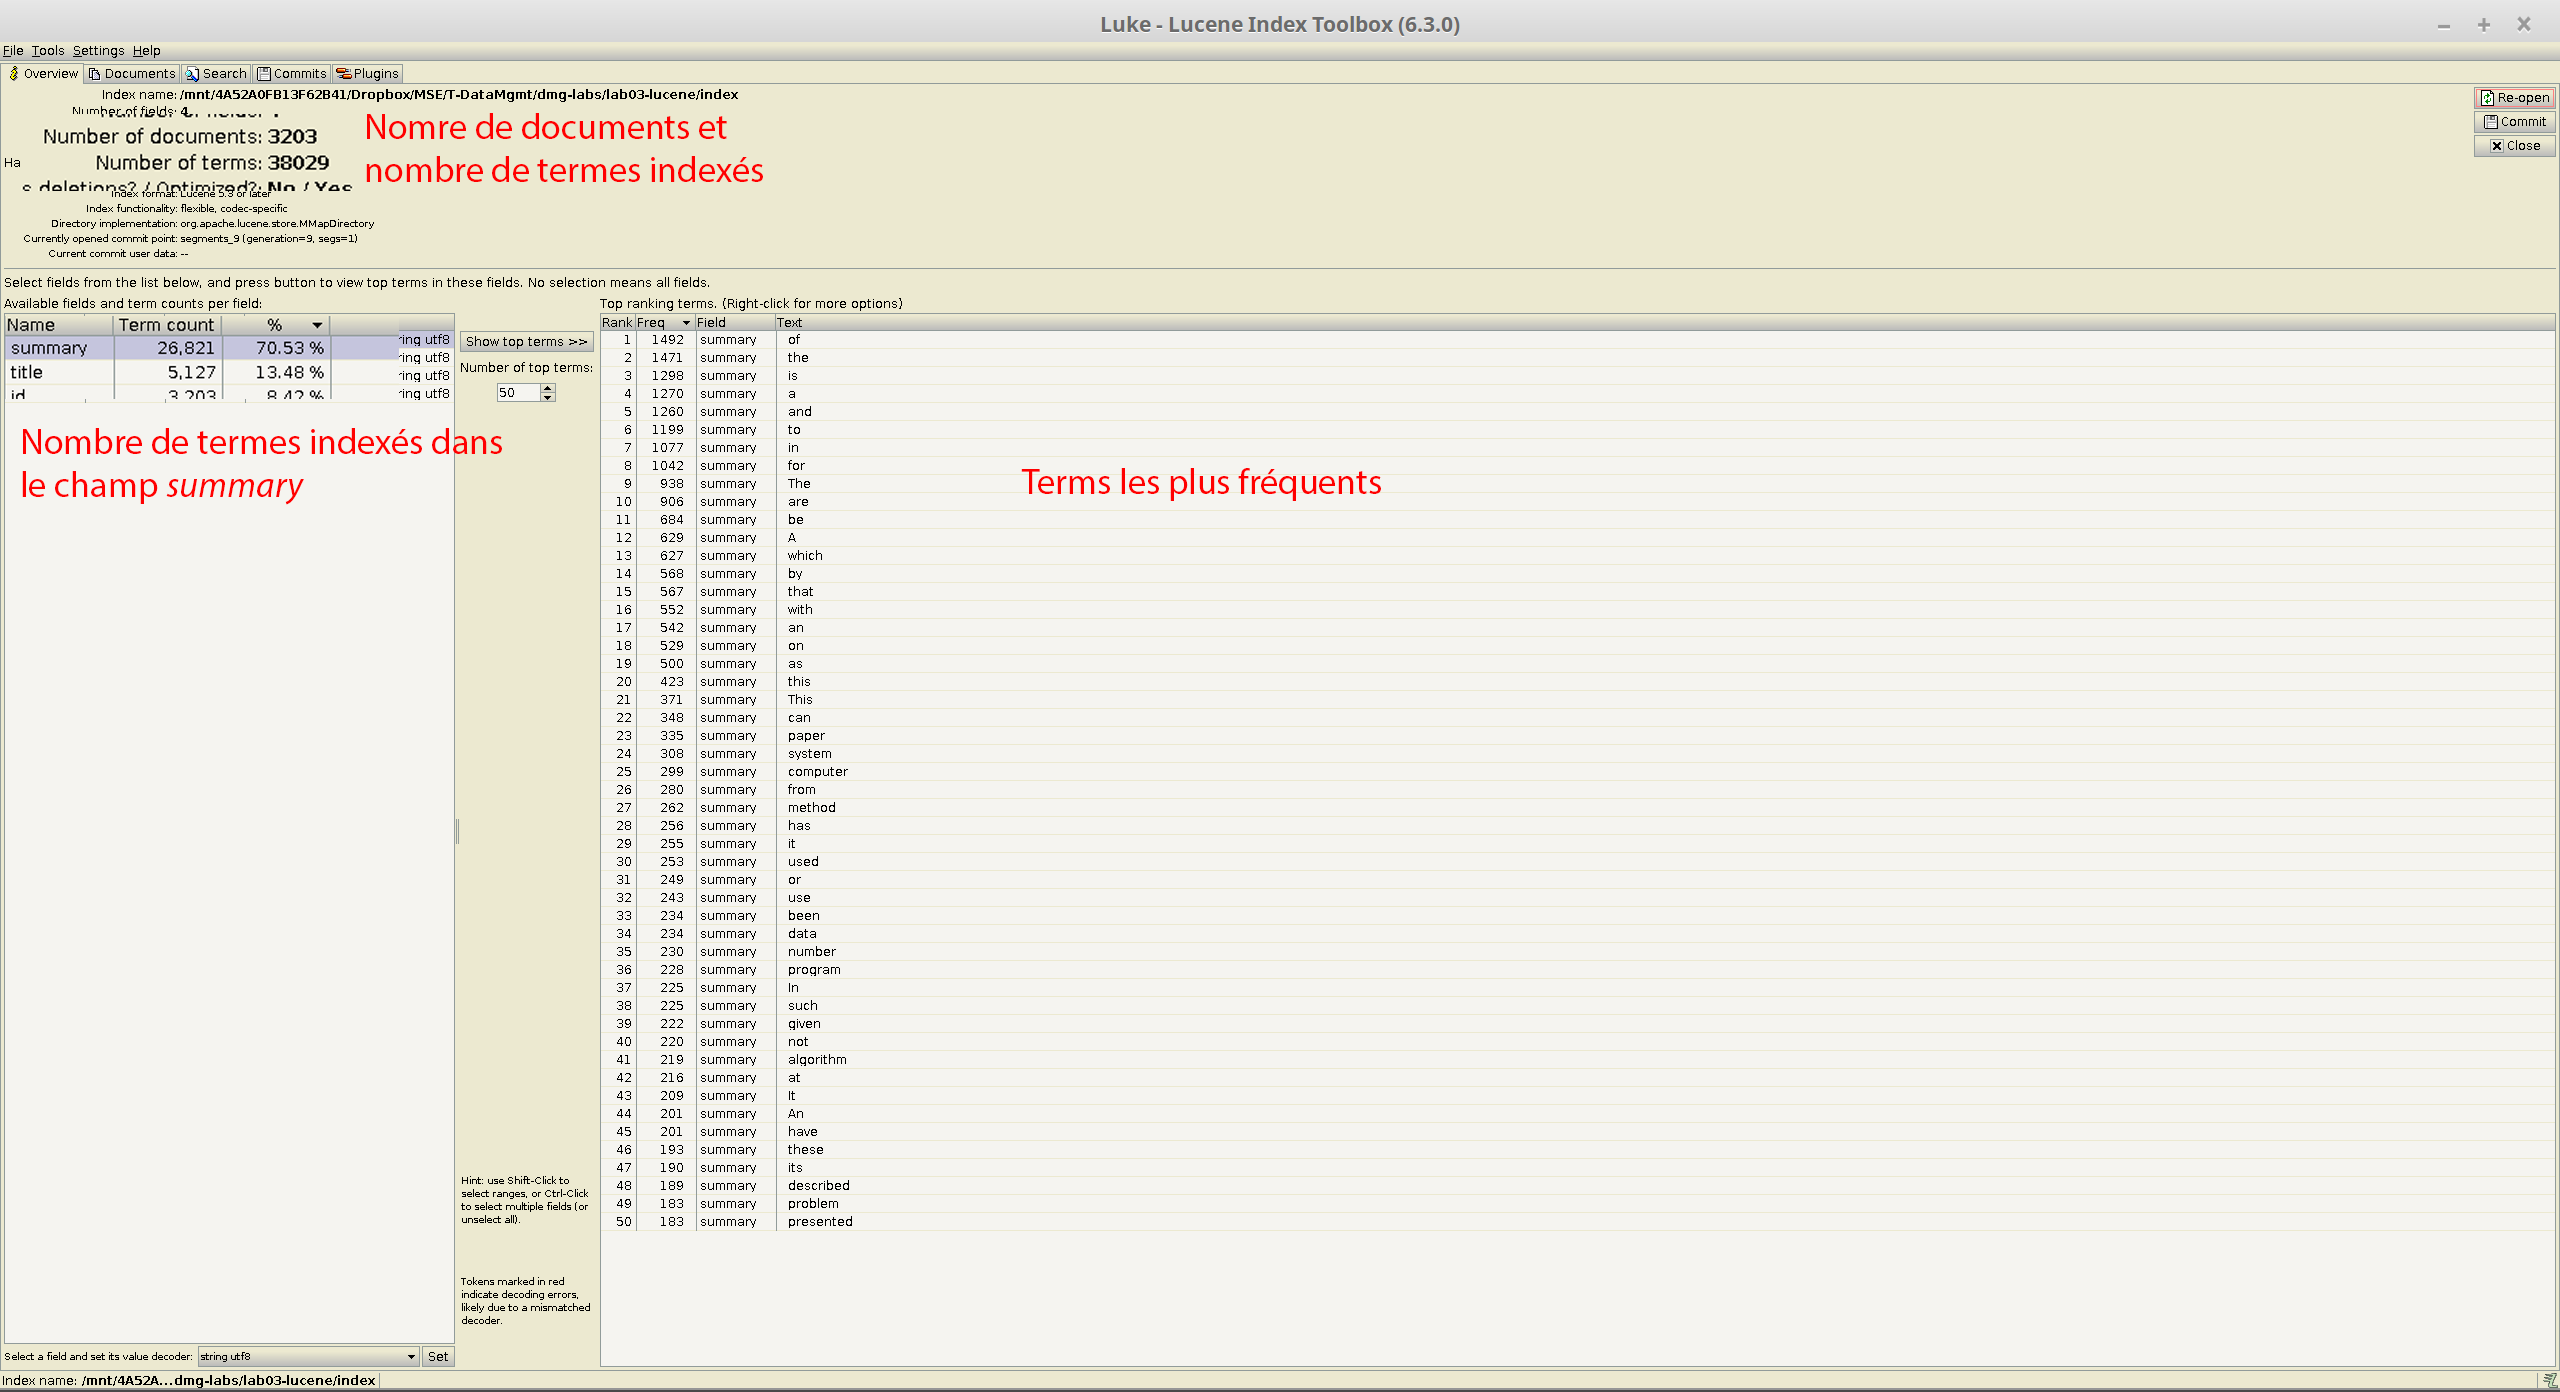
\includegraphics[width=1\linewidth, fbox]{img/Analyzers_White.png}
    \caption{Luke : WhitespaceAnalyzer exemple}
    \label{Analyzers_White}
\end{figure}

\subsection{EnglishAnalyzer}
\begin{enumerate}
    \item 3'203 / 26'212
    \item 16'724
    \item us / which / comput / program / system / present / describ / paper / method / can
    \item 2'388 kB
    \item 2'463 ms
\end{enumerate}

\subsection{ShingleAnalyzerWrapper (using shingle size 2)}
\begin{enumerate}
    \item 3'203 / 106'272
    \item 85'610
    \item which / system / paper / computer / can / " paper" / described / given / presented / time
    \item 5'449 kB
    \item 3'293 ms
\end{enumerate}

\subsection{ShingleAnalyzerWrapper (using shingle size 3)}
\begin{enumerate}
    \item 3'203 / 148'948
    \item 125'776
    \item which / system / computer / paper / can / described / time / given / presented / from
    \item 7'053 kB
    \item 3'580 ms
\end{enumerate}

\subsection{StopAnalyzer}
\begin{enumerate}
    \item 3'203 / 24'662
    \item 18.342
    \item system / computer / paper / presented / time / method / program / data / algorithm / discussed
    \item 2'214 kB
    \item 3'183 ms
\end{enumerate}

\section{Lecture de l'index}

Plutôt que d'utiliser Luke pour lire l'index, nous allons maintenant utiliser l'API Lucene. 

En utilisant la classe \textit{HighFreqTerms} nous devons répondre aux deux questions suivantes :

\textit{1. What is the author with the highest number of publications? How many publications does he/she have?}

Résultats :

\begin{center}
    \begin{tabular}{|l|r|}
      \hline
      Terms & Nb \\
      \hline
      Thacher Jr., H. C. & 38 \\
      Naur, P. & 19 \\
      Hill, I. D. & 16 \\
      Wirth, N. & 15 \\
      Pike, M. C. & 14 \\
      Herndon, J. R. & 14 \\
      Gautschi, W. & 14 \\
      Boothroyd, J. & 14 \\
      George, R. & 12 \\
      Floyd, R. W. & 12 \\
      Bemer, R. W. & 12 \\
      McKeeman, W. M. & 11 \\
      \hline
    \end{tabular}
\end{center}

Code :

\lstset{language=Java}
\begin{lstlisting}
public void authorWithMaxPublication() throws Exception {

Directory d = FSDirectory.open(FileSystems.getDefault().getPath("index"));
IndexReader ir = DirectoryReader.open(d);

HighFreqTerms.DocFreqComparator cmp = new HighFreqTerms.DocFreqComparator();
TermStats[] fields = HighFreqTerms.getHighFreqTerms(ir, 12, "author", cmp);
for (TermStats ts: fields)
    System.out.println(ts.termtext.utf8ToString() + " => " + ts.docFreq);

}
\end{lstlisting}

\textit{2. List the top 10 terms in the title field with their frequency.}

Résultats :

\begin{center}
    \begin{tabular}{|l|r|}
      \hline
      Terms & Nb \\
      \hline
      algorithm & 963 \\
      computer & 260 \\
      system & 172 \\
      programming & 154 \\
      method & 125 \\
      data & 110 \\
      systems & 108 \\
      language & 99 \\
      program & 93 \\
      matrix & 82 \\
      \hline
    \end{tabular}
\end{center}

Code :

\begin{lstlisting}
public void titleTermeTop() throws Exception {

Directory d = FSDirectory.open(FileSystems.getDefault().getPath("index"));
IndexReader ir = DirectoryReader.open(d);

HighFreqTerms.DocFreqComparator cmp = new HighFreqTerms.DocFreqComparator();
TermStats[] fields = HighFreqTerms.getHighFreqTerms(ir, 10, "title", cmp);
for (TermStats ts: fields)
    System.out.println(ts.termtext.utf8ToString() + " => " + ts.docFreq);

}
\end{lstlisting}

\section{Recherche}

Pour cette partie nous avons reconstruit notre index avec \textit{EnglishAnalyzer}.

Voici le prototype de notre fonction de requête :
\lstset{numbers=none}
\begin{lstlisting}
public void query(String fieldStr, String queryStr, String analyzer_type, int max_outputs) throws ParseException, IOException {...};
\end{lstlisting}

Voici les requêtes effectuées avec \textit{QueryParser} sur le champ \textit{summary} :

\begin{enumerate}

\item \textit{Publications containing the term "Information Retrieval".}

\begin{lstlisting}
cacm.query("summary", "Information Retrieval", analyzer_type, 10);
\end{lstlisting}

Voici les 10 premiers résultats de cette requête sur les \textbf{188} :

\begin{itemize}
    \item Query is: summary:inform summary:retriev
    \item 1457: Data Manipulation and Programming Problemsin Automatic Information Retrieval (8.651913)
    \item 891: Everyman's Information Retrieval System (8.181953)
    \item 1699: Experimental Evaluation of InformationRetrieval Through a Teletypewriter (7.5747085)
    \item 2307: Dynamic Document Processing (7.3587627)
    \item 3134: The Use of Normal Multiplication Tablesfor Information Storage and Retrieval (7.3557515)
    \item 1032: Theoretical Considerations in Information Retrieval Systems (7.312654)
    \item 1935: Randomized Binary Search Technique (7.1063213)
    \item 1681: Easy English,a Language for InformationRetrieval Through a Remote Typewriter Console (6.70207)
    \item 2990: Effective Information Retrieval Using Term Accuracy (6.70207)
    \item 2519: On the Problem of Communicating Complex Information (6.2497764)\\
\end{itemize}

\item \textit{Publications containing both "Information" and "Retrieval".}

\begin{lstlisting}
cacm.query("summary", "Information AND Retrieval", analyzer_type, 10);
\end{lstlisting}

Voici les 10 premiers résultats de cette requête sur les \textbf{23} :

\begin{itemize}
    \item Query is: +summary:inform +summary:retriev
    \item 1457: Data Manipulation and Programming Problemsin Automatic Information Retrieval (8.651913)
    \item 891: Everyman's Information Retrieval System (8.181953)
    \item 1699: Experimental Evaluation of InformationRetrieval Through a Teletypewriter (7.5747085)
    \item 2307: Dynamic Document Processing (7.3587627)
    \item 3134: The Use of Normal Multiplication Tablesfor Information Storage and Retrieval (7.3557515)
    \item 1032: Theoretical Considerations in Information Retrieval Systems (7.312654)
    \item 1935: Randomized Binary Search Technique (7.1063213)
    \item 1681: Easy English,a Language for InformationRetrieval Through a Remote Typewriter Console (6.70207)
    \item 2990: Effective Information Retrieval Using Term Accuracy (6.70207)
    \item 2519: On the Problem of Communicating Complex Information (6.2497764)\\
\end{itemize}

\item \textit{Publications containing at least the term "Retrieval" and, possibly "Information" but not "Database".}

\begin{lstlisting}
cacm.query("summary", "+Retrieval Information -Database", analyzer_type, 10);
\end{lstlisting}

Voici les 10 premiers résultats de cette requête sur les \textbf{54} :

\begin{itemize}
    \item Query is: +summary:retriev summary:inform -summary:databas
    \item 1457: Data Manipulation and Programming Problemsin Automatic Information Retrieval (8.651913)
    \item 891: Everyman's Information Retrieval System (8.181953)
    \item 1699: Experimental Evaluation of InformationRetrieval Through a Teletypewriter (7.5747085)
    \item 2307: Dynamic Document Processing (7.3587627)
    \item 3134: The Use of Normal Multiplication Tablesfor Information Storage and Retrieval (7.3557515)
    \item 1032: Theoretical Considerations in Information Retrieval Systems (7.312654)
    \item 1935: Randomized Binary Search Technique (7.1063213)
    \item 1681: Easy English,a Language for InformationRetrieval Through a Remote Typewriter Console (6.70207)
    \item 2990: Effective Information Retrieval Using Term Accuracy (6.70207)
    \item 2519: On the Problem of Communicating Complex Information (6.2497764)\\
\end{itemize}

\item \textit{Publications containing a term starting with "Info".}

\begin{lstlisting}
cacm.query("summary", "Info*", analyzer_type, 10);
\end{lstlisting}

Voici les 10 premiers résultats de cette requête sur les \textbf{193} :

\begin{itemize}
    \item Query is: summary:info*
    \item 222: Coding Isomorphisms (1.0)
    \item 272: A Storage Allocation Scheme for ALGOL 60 (1.0)
    \item 396: Automation of Program  Debugging (1.0)
    \item 397: A Card Format for Reference Files in Information Processing (1.0)
    \item 409: CL-1, An Environment for a Compiler (1.0)
    \item 440: Record Linkage (1.0)
    \item 483: On the Nonexistence of a Phrase Structure Grammar for ALGOL 60 (1.0)
    \item 616: An Information Algebra - Phase I Report-LanguageStructure Group of the CODASYL Development Committee (1.0)
    \item 644: A String Language for Symbol Manipulation Based on ALGOL 60 (1.0)
    \item 655: COMIT as an IR Language (1.0)\\
\end{itemize}

\item \textit{Publications containing the term "Information" close to "Retrieval" (max distance 5).}

\begin{lstlisting}
cacm.query("summary", "'Information Retrieval'~5", analyzer_type, 10);
\end{lstlisting}

Voici les 10 premiers résultats de cette requête sur les \textbf{159} :

\begin{itemize}
    \item Query is: summary:inform summary:retrieval'~2
    \item 2160: Canonical Structure in Attribute Based File Organization (11.125051)
    \item 2832: Faster Retrieval from Context Trees (Corrigendum) (5.5161905)
    \item 1516: Automatic Data Compression (4.020056)
    \item 1746: Protection in an Information Processing Utility (4.0018125)
    \item 2870: A Lattice Model of Secure Information Flow (3.8555226)
    \item 1267: Performance of Systems Used for Data TransmissionTransfer Rate of Information Bits -An ASA TutorialStandard (3.8451033)
    \item 3134: The Use of Normal Multiplication Tablesfor Information Storage and Retrieval (3.7823412)
    \item 2905: Perfect Hashing Functions: A SingleProbe Retrieving Method for Static Sets (3.6556962)
    \item 1457: Data Manipulation and Programming Problemsin Automatic Information Retrieval (3.5519412)
    \item 1745: A Position Paper on Computing and Communications (3.5519412)\\
\end{itemize}

\end{enumerate}

\section{Améliorer le Score de Lucene}

Nous exécutons la première requête du point précédent (\textit{Information Retrieval} avec \textit{EnglishAnalysez}) avec la fonction de similarité par défaut et ensuite avec une fonction customisée.

Le code de la fonction similarité customisée :
\lstset{numbers=left}
\begin{lstlisting}
package cacm;

import org.apache.lucene.index.FieldInvertState;
import org.apache.lucene.search.similarities.ClassicSimilarity;

public class CustomSimilarity extends ClassicSimilarity {

    @Override
    public float tf(float freq) {
        return (float) (1 + Math.log((double) freq));
    }

    @Override
    public float idf(long docFreq, long numDocs) {
        return (float) Math.log(numDocs / docFreq);
    }

    @Override
    public float coord(int overlap, int maxOverlap) {
        return (float) Math.sqrt(overlap / maxOverlap);
    }

    @Override
    public float lengthNorm(FieldInvertState state) {
        return 1f;
    }
}
\end{lstlisting}

Le code suivant ajoute cette classe au moment de l'indexation :
\begin{lstlisting}
IndexWriterConfig iwc = new IndexWriterConfig(index_analyzer);
iwc.setOpenMode(IndexWriterConfig.OpenMode.CREATE);
iwc.setUseCompoundFile(false);
iwc.setSimilarity(new CustomSimilarity());
\end{lstlisting}

Et ce code au moment de la recherche :
\begin{lstlisting}
IndexSearcher indexSearcher = new IndexSearcher(indexReader);
indexSearcher.setSimilarity(new CustomSimilarity());
\end{lstlisting}

Voici les 10 premiers résultats avec la fonction de similarité par défaut avec le score entre paranthèses :

\begin{itemize}
    \item 1457: Data Manipulation and Programming Problemsin Automatic Information Retrieval (8.651913)
    \item 891: Everyman's Information Retrieval System (8.181953)
    \item 1699: Experimental Evaluation of InformationRetrieval Through a Teletypewriter (7.5747085)
    \item 2307: Dynamic Document Processing (7.3587627)
    \item 3134: The Use of Normal Multiplication Tablesfor Information Storage and Retrieval (7.3557515)
    \item 1032: Theoretical Considerations in Information Retrieval Systems (7.312654)
    \item 1935: Randomized Binary Search Technique (7.1063213)
    \item 1681: Easy English,a Language for InformationRetrieval Through a Remote Typewriter Console (6.70207)
    \item 2990: Effective Information Retrieval Using Term Accuracy (6.70207)
    \item 2519: On the Problem of Communicating Complex Information (6.2497764)
\end{itemize}

Et voici maintenant les 10 premiers résultats avec la fonction de similarité customisée :

\begin{itemize}
    \item 1032: Theoretical Considerations in Information Retrieval Systems (8.500153)
    \item 1457: Data Manipulation and Programming Problemsin Automatic Information Retrieval (8.500153)
    \item 3134: The Use of Normal Multiplication Tablesfor Information Storage and Retrieval (8.295944)
    \item 891: Everyman's Information Retrieval System (7.9694023)
    \item 1699: Experimental Evaluation of InformationRetrieval Through a Teletypewriter (7.9694023)
    \item 2307: Dynamic Document Processing (7.3886204)
    \item 1681: Easy English,a Language for InformationRetrieval Through a Remote Typewriter Console (7.0620785)
    \item 2990: Effective Information Retrieval Using Term Accuracy (7.0620785)
    \item 1527: A Grammar Base Question Answering Procedure (6.8578696)
    \item 1652: A Code for Non-numeric Information ProcessingApplications in Online Systems (5.865016)
\end{itemize}

Et l'on observe très bien des différents scores sur les documents. Ceux avec la fonction customisée sont plus élevé.

Nous avons vu dans la donnée de ce laboratoire que le score était calculé par défaut selon cette formule:

\begin{equation}
score(q,d)=\sum [tf(t_{d}) \times idf(t) \times boost(t.field_{d}) \times norm(t,d)] \times coord(q,d) \times qNorm(q)
\end{equation}

Dans la classe \texttt{CustomSimilarity}, quatre méthodes ont été réécrites et ont prit la place des méthodes par défaut selon le tableau ci-dessous.

\begin{center}
  \begin{tabular}{|r|c|c|}
    \hline
    & \texttt{ClassicSimilarity} & \texttt{CustomSimilarity} \\
    \hline
    \texttt{tf()} & $sqrt(freq)$ & $1+log(freq)$ \\
    \hline
    \texttt{idf()} & $log((numDocs+1)/(docFreq+1))+1$ & $log(numDocs/docFreq)$ \\
    \hline
    \texttt{coord()} & $overlap/maxOverlap$ & $sqrt(overlap/maxOverlap)$ \\
    \hline
    \texttt{lengthNorm()} &$state.getBoost()*1/sqrt(numTerms)))$ & $1$ \\
    \hline
  \end{tabular}
\end{center}

Dans la fonction de calcul du score ci-dessus, ces modifications ont les influences suivantes: \\

\begin{itemize}
  \item $tf(t_{d})$ sera très amortie dans \texttt{CustomSimilarity}
    \begin{figure}[h]
        \centering
        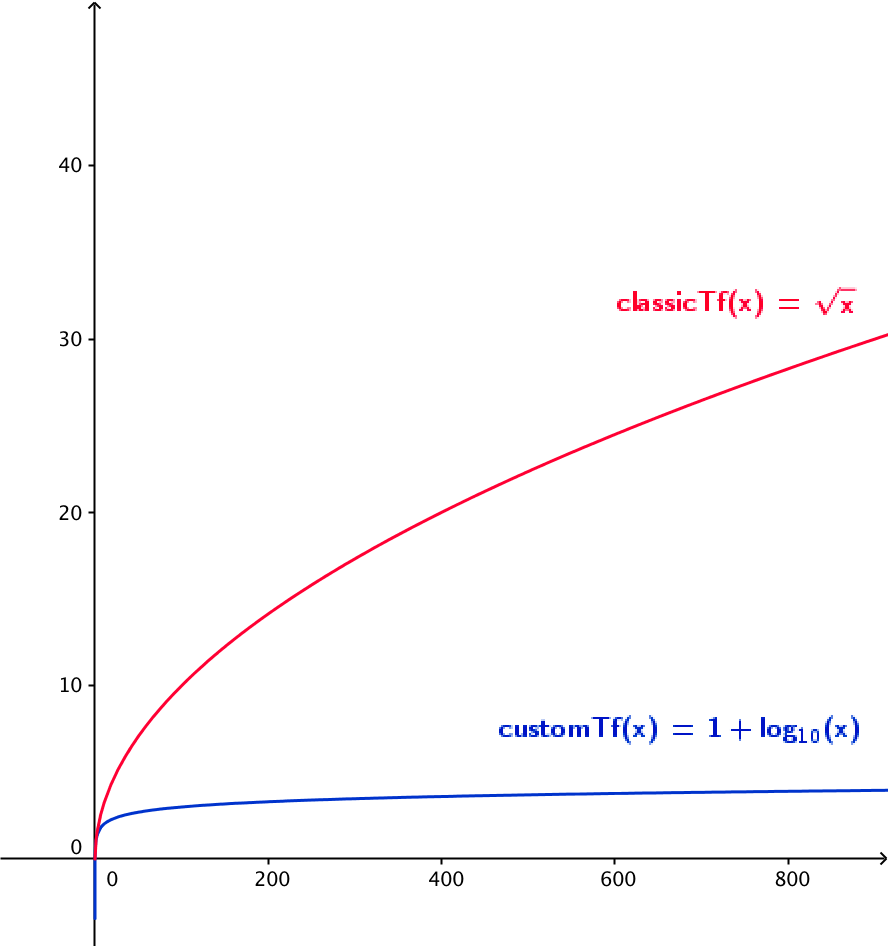
\includegraphics[width=0.4\linewidth]{img/tf.png}
        \caption{Plot des fréquences de termes}
        \label{tfplot}
    \end{figure}

  \item $idf(t)$ sera très amortie dans \texttt{CustomSimilarity}, ceci est majoritairement dû à son ordonnée qui n'a plus d'offset.\footnote{3203 est le nombre de documents dans \texttt{cacm.txt}}
    \begin{figure}[h]
        \centering
        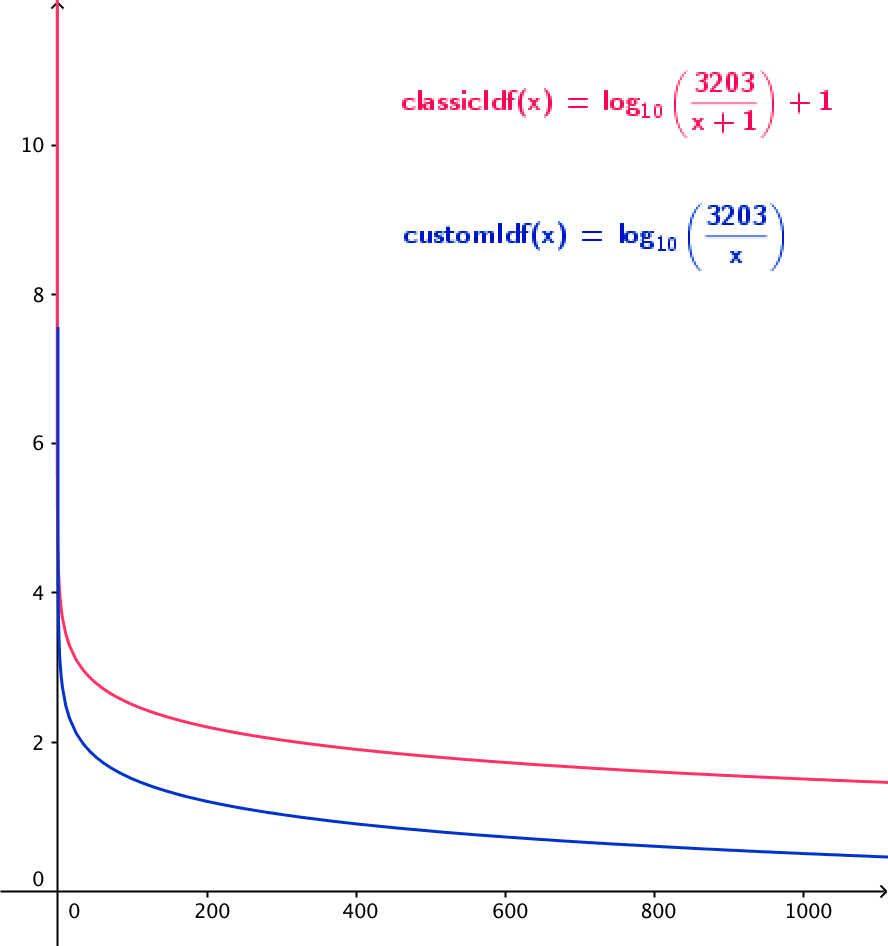
\includegraphics[width=0.4\linewidth]{img/idf.png}
        \caption{Plot des fréquences documentaires inversée}
        \label{idfplot}
    \end{figure}

  \item $coord(q,d)$ est plus faible dans \texttt{CustomSimilarity} car $overlap/maxOverlap$ est mis à la racine.
  \item le terme $norm(t,d)$ n'a plus d'influence sur le score car il est remplacé par 1.\\
\end{itemize}

L'obtention d'un score final plus élevé avec le scorrer \texttt{CustomSimilarity} est expliquée par le dernier point. Par défaut, les valeurs que prendra $norm(t,d)$
vont dépendre de $boost*1/sqrt(numTerms)))$. On constate qu'à moins que $boost$ soit plus grand que $sqrt(numTerms)$, $norm(t,d)$ sera compris entre 0 et 1. Dans notre cas, nous n'avons pas appliqué de boost lors de l'indexation et le nombre de termes est égal à 3203 dans notre corpus. Le résultat prendra donc une valeur de $1*1/sqrt(3203) \approx 0.018$.
